\RequirePackage{atbegshi}
\documentclass[compress,aspectratio=169,usenames,dvipsnames]{beamer}\usepackage[]{graphicx}\usepackage[]{xcolor}
% maxwidth is the original width if it is less than linewidth
% otherwise use linewidth (to make sure the graphics do not exceed the margin)
\makeatletter
\def\maxwidth{ %
  \ifdim\Gin@nat@width>\linewidth
    \linewidth
  \else
    \Gin@nat@width
  \fi
}
\makeatother

\definecolor{fgcolor}{rgb}{0.345, 0.345, 0.345}
\newcommand{\hlnum}[1]{\textcolor[rgb]{0.686,0.059,0.569}{#1}}%
\newcommand{\hlstr}[1]{\textcolor[rgb]{0.192,0.494,0.8}{#1}}%
\newcommand{\hlcom}[1]{\textcolor[rgb]{0.678,0.584,0.686}{\textit{#1}}}%
\newcommand{\hlopt}[1]{\textcolor[rgb]{0,0,0}{#1}}%
\newcommand{\hlstd}[1]{\textcolor[rgb]{0.345,0.345,0.345}{#1}}%
\newcommand{\hlkwa}[1]{\textcolor[rgb]{0.161,0.373,0.58}{\textbf{#1}}}%
\newcommand{\hlkwb}[1]{\textcolor[rgb]{0.69,0.353,0.396}{#1}}%
\newcommand{\hlkwc}[1]{\textcolor[rgb]{0.333,0.667,0.333}{#1}}%
\newcommand{\hlkwd}[1]{\textcolor[rgb]{0.737,0.353,0.396}{\textbf{#1}}}%
\let\hlipl\hlkwb

\usepackage{framed}
\makeatletter
\newenvironment{kframe}{%
 \def\at@end@of@kframe{}%
 \ifinner\ifhmode%
  \def\at@end@of@kframe{\end{minipage}}%
  \begin{minipage}{\columnwidth}%
 \fi\fi%
 \def\FrameCommand##1{\hskip\@totalleftmargin \hskip-\fboxsep
 \colorbox{shadecolor}{##1}\hskip-\fboxsep
     % There is no \\@totalrightmargin, so:
     \hskip-\linewidth \hskip-\@totalleftmargin \hskip\columnwidth}%
 \MakeFramed {\advance\hsize-\width
   \@totalleftmargin\z@ \linewidth\hsize
   \@setminipage}}%
 {\par\unskip\endMakeFramed%
 \at@end@of@kframe}
\makeatother

\definecolor{shadecolor}{rgb}{.97, .97, .97}
\definecolor{messagecolor}{rgb}{0, 0, 0}
\definecolor{warningcolor}{rgb}{1, 0, 1}
\definecolor{errorcolor}{rgb}{1, 0, 0}
\newenvironment{knitrout}{}{} % an empty environment to be redefined in TeX

\usepackage{alltt} % aspectratio=169


% % % % % % % % % % % % % % %
%             MY PACKAGES 
% % % % % % % % % % % % % % %
\usepackage{graphicx}       % Use pdf, png, jpg, or eps with pdflatex; use eps in DVI mode
\usepackage{dcolumn} % this pack is neccesary to build nicer columns with texreg--dont remove it.
\usepackage[export]{adjustbox}
\usepackage{xcolor}[dvipsnames]
\usepackage{amssymb,amsmath}
\usepackage{threeparttable} % package to have long notes in reg tables in texreg. 
\usepackage{graphics}
\usepackage{pgfplots}
\pgfplotsset{compat=1.11}
\usepgfplotslibrary{fillbetween}
\usepackage{fontawesome}


%\usepackage{tipx}
%\usepackage{tikz}
%\usetikzlibrary{arrows,shapes,decorations.pathmorphing,backgrounds,positioning,fit,petri}
\usepackage{rotating}
%\usepackage{scalerel} % for inline images
\usepackage{import}
%\usepackage{times}
\usepackage{array}
\usepackage{tabularx}
\usepackage{booktabs}
%\usepackage{textcomp}
\usepackage{float}
%\usepackage{setspace}      % \doublespacing \singlespacing \onehalfspacing %doble espacio
%\label{x:y}                          %ocupar para autoref.
%\autoref{x:y}                        %ocupar para autoref.
%\usepackage{nopageno}      %desactivar para p�ginas
\usepackage{pifont}
\newcommand{\xmark}{\ding{55}}%

%\usepackage{marvosym} %faces

\usepackage{hyperref}
\hypersetup{
    %bookmarks=true,         % show bookmarks bar?
    unicode=false,          % non-Latin characters in Acrobat’s bookmarks
    pdftoolbar=true,        % show Acrobat’s toolbar?
    pdfmenubar=true,        % show Acrobat’s menu?
    pdffitwindow=true,     % window fit to page when opened
    pdfstartview={FitH},    % fits the width of the page to the window
    pdftitle={My title},    % title
    pdfauthor={Author},     % author
    pdfsubject={Subject},   % subject of the document
    pdfcreator={Creator},   % creator of the document
    pdfproducer={Producer}, % producer of the document
    pdfkeywords={keyword1} {key2} {key3}, % list of keywords
    pdfnewwindow=true,      % links in new window
    colorlinks=true,       % false: boxed links; true: colored links
    linkcolor=blue,          % color of internal links (change box color with linkbordercolor)
    citecolor=blue,        % color of links to bibliography
    filecolor=blue,      % color of file links
    urlcolor=blue           % color of external links
}

\hypersetup{
  colorlinks = true,
  urlcolor = blue,
  pdfpagemode = UseNone
}


\usepackage{multirow}

\usepackage{tikz}
\usetikzlibrary{arrows,decorations.pathreplacing}



\usepackage{listings}
\usepackage{color}
\definecolor{amber}{rgb}{1.0, 0.75, 0.0}
\definecolor{americanrose}{rgb}{1.0, 0.01, 0.24}
\definecolor{dkgreen}{rgb}{0,0.6,0}
\definecolor{gray}{rgb}{0.5,0.5,0.5}
\definecolor{mauve}{rgb}{0.58,0,0.82}
\lstset{ %
  language=R,                     % the language of the code
  basicstyle=\TINY,           % the size of the fonts that are used for the code
  numbers=left,                   % where to put the line-numbers
  numberstyle=\tiny\color{gray},  % the style that is used for the line-numbers
  stepnumber=1,                   % the step between two line-numbers. If it's 1, each line
                                  % will be numbered
  numbersep=5pt,                  % how far the line-numbers are from the code
  backgroundcolor=\color{white},  % choose the background color. You must add \usepackage{color}
  showspaces=false,               % show spaces adding particular underscores
  showstringspaces=false,         % underline spaces within strings
  showtabs=false,                 % show tabs within strings adding particular underscores
  frame=single,                   % adds a frame around the code
  rulecolor=\color{black},        % if not set, the frame-color may be changed on line-breaks within not-black text (e.g. commens (green here))
  tabsize=1,                      % sets default tabsize to 2 spaces
  captionpos=b,                   % sets the caption-position to bottom
  breaklines=true,                % sets automatic line breaking
  breakatwhitespace=false,        % sets if automatic breaks should only happen at whitespace
  title=\lstname,                 % show the filename of files included with \lstinputlisting;
                                  % also try caption instead of title
  keywordstyle=\color{blue},      % keyword style
  commentstyle=\color{dkgreen},   % comment style
  stringstyle=\color{mauve},      % string literal style
  escapeinside={\%*}{*)},         % if you want to add a comment within your code
  morekeywords={*,...}            % if you want to add more keywords to the set
} 

% % % % % % % % % % % % % % %
%           PACKAGE CUSTOMIZATION
% % % % % % % % % % % % % % %

% GENERAL CUSTOMIZATION
\usepackage[math]{iwona}% font
\usetheme{Singapore}  % template I should use
%\usetheme{Szeged}  % alternative template
\usecolortheme{rose}  % color template
\makeatletter     % to show subsection/section title (1/3)
\beamer@theme@subsectiontrue % to show subsection/section title (2/3)
\makeatother      % to show subsection/section title (3/3)



% THIS BELOW IS TO MAKE NAVIGATION DOTS MARKED DURING PRESENTATION
\makeatletter
\def\slideentry#1#2#3#4#5#6{%
  %section number, subsection number, slide number, first/last frame, page number, part number
  \ifnum#6=\c@part\ifnum#2>0\ifnum#3>0%
    \ifbeamer@compress%
      \advance\beamer@xpos by1\relax%
    \else%
      \beamer@xpos=#3\relax%
      \beamer@ypos=#2\relax%
    \fi%
  \hbox to 0pt{%
    \beamer@tempdim=-\beamer@vboxoffset%
    \advance\beamer@tempdim by-\beamer@boxsize%
    \multiply\beamer@tempdim by\beamer@ypos%
    \advance\beamer@tempdim by -.05cm%
    \raise\beamer@tempdim\hbox{%
      \beamer@tempdim=\beamer@boxsize%
      \multiply\beamer@tempdim by\beamer@xpos%
      \advance\beamer@tempdim by -\beamer@boxsize%
      \advance\beamer@tempdim by 1pt%
      \kern\beamer@tempdim
      \global\beamer@section@min@dim\beamer@tempdim
      \hbox{\beamer@link(#4){%
          \usebeamerfont{mini frame}%
          \ifnum\c@section>#1%
            %\usebeamercolor[fg]{mini frame}%
            %\usebeamertemplate{mini frame}%
            \usebeamercolor{mini frame}%
            \usebeamertemplate{mini frame in other subsection}%
          \else%
            \ifnum\c@section=#1%
              \ifnum\c@subsection>#2%
                \usebeamercolor[fg]{mini frame}%
                \usebeamertemplate{mini frame}%
              \else%
                \ifnum\c@subsection=#2%
                  \usebeamercolor[fg]{mini frame}%
                  \ifnum\c@subsectionslide<#3%
                    \usebeamertemplate{mini frame in current subsection}%
                  \else%
                    \usebeamertemplate{mini frame}%
                  \fi%
                \else%
                  \usebeamercolor{mini frame}%
                  \usebeamertemplate{mini frame in other subsection}%
                \fi%
              \fi%
            \else%
              \usebeamercolor{mini frame}%
              \usebeamertemplate{mini frame in other subsection}%
            \fi%
          \fi%
        }}}\hskip-10cm plus 1fil%
  }\fi\fi%
  \else%
  \fakeslideentry{#1}{#2}{#3}{#4}{#5}{#6}%
  \fi\ignorespaces
  }
\makeatother


%%% bib begin
\usepackage[authordate,isbn=false,doi=false,url=false,eprint=false]{biblatex-chicago}
\DeclareFieldFormat[article]{title}{\mkbibquote{#1}} % make article titles in quotes
\DeclareFieldFormat[thesis]{title}{\mkbibemph{#1}} % make theses italics

\AtEveryBibitem{\clearfield{month}}
\AtEveryCitekey{\clearfield{month}}

\addbibresource{/Users/hectorbahamonde/Bibliografia_PoliSci/library.bib} 


% USAGES
%% use \textcite to cite normal
%% \parencite to cite in parentheses
%% \footcite to cite in footnote
%% the default can be modified in autocite=FOO, footnote, for ex. 
%%% bib end



% % % % % % % % % % % % % % %
%       To show the TITLE at the Bottom of each slide
% % % % % % % % % % % % % % %

\beamertemplatenavigationsymbolsempty 
\makeatletter
\setbeamertemplate{footline}
{
\leavevmode%
\hbox{%
\begin{beamercolorbox}[wd=1\paperwidth,ht=2.25ex,dp=2ex,center]{title in head/foot}%
\usebeamerfont{title in head/foot}\insertshorttitle
\end{beamercolorbox}%
\begin{beamercolorbox}[wd=1
\paperwidth,ht=2.25ex,dp=2ex,center]{date in head/foot}%
\end{beamercolorbox}}%
}
\makeatother



% to switch off navigation bullets
%% using \miniframeson or \miniframesoff
\makeatletter
\let\beamer@writeslidentry@miniframeson=\beamer@writeslidentry
\def\beamer@writeslidentry@miniframesoff{%
  \expandafter\beamer@ifempty\expandafter{\beamer@framestartpage}{}% does not happen normally
  {%else
    % removed \addtocontents commands
    \clearpage\beamer@notesactions%
  }
}
\newcommand*{\miniframeson}{\let\beamer@writeslidentry=\beamer@writeslidentry@miniframeson}
\newcommand*{\miniframesoff}{\let\beamer@writeslidentry=\beamer@writeslidentry@miniframesoff}
\makeatother

% Image full size: use 
%%\begin{frame}
  %%\fullsizegraphic{monogram.jpg}
%%\end{frame}
\newcommand<>{\fullsizegraphic}[1]{
  \begin{textblock*}{0cm}(-1cm,-3.78cm)
  \includegraphics[width=\paperwidth]{#1}
  \end{textblock*}
}


% hyperlinks
\hypersetup{colorlinks,
            urlcolor=[rgb]{0.01, 0.28, 1.0},
            linkcolor=[rgb]{0.01, 0.28, 1.0}}



%\newcommand{\vitem}[]{\vfill \item}

% % % % % % % % % % % % % % %
%           DOCUMENT ID
% % % % % % % % % % % % % % %

\title{\input{title.txt}\unskip} % 




\author[shortname]{
Hector Bahamonde \inst{1} \and 
Inga Saikkonen \inst{2} \and 
Mart Trasberg \inst{3} \\ \vspace{3mm} \scriptsize{\color{gray}Authors in alphabetical order. All contributed equally to this paper.}
}

\institute[shortinst]{\inst{1} University of Turku, Finland \and %
                      \inst{2} \textnormal{Åbo Akademi}, Finland \and
                      \inst{3} Tecn\'ologico de Monterrey, Mexico}




\date{\today}

%to to see shadows of previous blocks
%\setbeamercovered{dynamic}
\IfFileExists{upquote.sty}{\usepackage{upquote}}{}
\begin{document}





\begin{knitrout}
\definecolor{shadecolor}{rgb}{0.969, 0.969, 0.969}\color{fgcolor}
\end{knitrout}

% % % % % % % % % % % % % % %
%           CONTENT
% % % % % % % % % % % % % % %

%% title frame
\begin{frame}
\titlepage
\end{frame}


\section{Introduction}


\subsection{Motivation}

\miniframeson
\begin{frame}[c]{``Losers' Consent'': A Weak Assumption}
\begin{columns}[T] % The [T] option aligns column content at the top

    \begin{column}{0.5\textwidth} % Left column and width
        \begin{itemize}
            \item<1-> Political elites in stable democracies typically accept electoral losses.
            \item<2-> Yet, actions by Trump's and Bolsonaro's supporters seriously questioned their acceptance of defeat.
            \item<3-> Research has looked into ``losers' consent,'' focusing on satisfaction, trust, and efficacy.
            \item<4-> Still, {\bf we know little about voters' ``systemic support'' when they lose elections} \scriptsize{{\color{gray}(Easton, 1965)}}.
        \end{itemize}
    \end{column}

    \begin{column}{0.5\textwidth} % Right column and width
        % Show the first figure only with the first item
        \begin{figure}
            \includegraphics<2,3,4>[scale=0.4]{Brasil_US_storming.jpeg} % Adjust path and size as needed
        \end{figure}
    \end{column}
    
\end{columns}
\end{frame}


\subsection{Our Paper}

\miniframeson
\begin{frame}[c]{Voters' Commitment:}
\framesubtitle{Electoral Losses and Institutional Heterogeneities}

  \begin{itemize}
    \item We analyze the level of system support among electoral ``losers'' using novel data from a conjoint experiment in Chile (N=811) and Estonia (N=639).

    \item We exploit institutional heterogeneities in presidential and parliamentary systems, which effectively shift the \emph{costs} of losing/winning an election.

    \item We pre-registered the following hypotheses: \href{https://osf.io/u72z4}{\beamergotobutton{\texttt{link}}}
      
    \begin{itemize}
      \item[H1] \only<1>{Electoral ``losers'' favor candidates endorsing anti-systemic actions more than ``winners.''}\only<3>{Election ``losers'' favor candidates endorsing anti-systemic actions more than ``winners.''}
           \only<2>{\textcolor{americanrose}{Election ``losers'' favor candidates endorsing anti-systemic actions more than ``winners.''}}
      \item[H2] \only<1-2>{This tendency is stronger in presidential versus parliamentary systems.}
           \only<3>{\textcolor{amber}{This tendency is stronger in presidential versus parliamentary systems.}}
    \end{itemize}

\end{itemize}

\end{frame}

\section{Theory}

\subsection{Soc. Movements and Institutional Literature}



\miniframeson
\begin{frame}[c]{Voters' Commitment:}
\framesubtitle{Electoral Losses and Institutional Heterogeneities}

  \begin{enumerate}
    \item Citizens' support for violent protests varies between electoral winners and losers.

      \begin{itemize}
        
        \item \emph{``Angry'' losers} might be more willing to support anti-systemic politicians {\tiny{\color{gray}(Bowler, Donovan, and Karp 2007)}}.
 
        \item Winners should oppose politicians supporting anti-systemic actions.
     
      \end{itemize}

  \item Institutional setting should affect differently the costs of losing an election \tiny{{\color{gray}(Lijphart, 2012)}}.

        \begin{itemize}
        
        \item  {\bf Presidential}: losers have little input outside of the electoral cycle. 

        \item {\bf Parliamentary}: losers’ interests can be represented through a variety of power sharing institutions. 
     
      \end{itemize}

\end{enumerate}

\end{frame}



\section{Research Design}

\subsection{Case Selection}

\miniframeson
\begin{frame}[c]{Losers' Consent and Democratic Stability}


\begin{columns}

\onslide<1->{
\begin{column}[T]{0.45\textwidth}
    \begin{minipage}[c][.6\textheight][c]{\linewidth}
    \begin{itemize}
        \item Collected novel data from Chile (N=811) and Estonia (N=639) with gender and party sample quotas.

        \item {\bf Most dissimilar cases}: maximize variance regarding government system (Presidential and Parliamentary).

        \item {\bf Most similar cases}: minimize variance regarding critical V-Dem variables.
    \end{itemize} 
    \end{minipage}}
\end{column}

\begin{column}[T]{0.65\textwidth}
    \begin{minipage}[c][.6\textheight][c]{1.1\linewidth}
    \centering{\includegraphics<2>[width=.51\textwidth]{VD_Chile_Estonia_ElecFree.pdf}}
    \centering{\includegraphics<3>[width=.51\textwidth]{VD_Chile_Estonia_LosersConsent.pdf}}
    \centering{\includegraphics<4>[width=.51\textwidth]{VD_Chile_Estonia_FreedomAssam.pdf}}
    \end{minipage}
\end{column}

\end{columns}

\end{frame}



\subsection{Experimental Design}

\miniframeson
\begin{frame}[c]{Conjoint Experiment}

  \begin{itemize}
    \item Designed an unconstrained, fully randomized conjoint experiment. %{\tiny\parencite{Hainmueller2014}}.
    \item We depart from standard AMCE analyses {\scriptsize\parencite{Hainmueller2014}} and instead compute {\bf subgroup marginal means} {\scriptsize\parencite{Leeper2020a}}.
    %\item In practice, when using marginal means, there's no need to set a reference category.
    %\item ``In a forced-choice conjoint design, the grand mean is by definition 0.5'' {\scriptsize\parencite[p. 209]{Leeper2020a}}.

  \end{itemize}


\begin{table}[h]
%\begin{footnotesize}
\scalebox{0.7}{
\begin{tabular}{  c |  p{0.6\linewidth} }
\toprule
\textbf{Dimension} & \textbf{Attribute Set} \\
\midrule
{\only<2,3>{\leavevmode\color{blue}}Gender} & {\only<2>{\leavevmode\color{red}}Male}, {\only<3>{\leavevmode\color{red}}Female}. \\
{\only<4,5,6>{\leavevmode\color{blue}}Age} & {\only<4>{\leavevmode\color{red}}Younger than 35}, {\only<5>{\leavevmode\color{red}}Between 35-50}, {\only<6>{\leavevmode\color{red}}Over 50}. \\
{\only<7,8>{\leavevmode\color{blue}}Protest} & {\only<7>{\leavevmode\color{red}}The candidate OPPOSES anti-government protest that will seek to de-destabilize the current government}, {\only<8>{\leavevmode\color{red}}The candidate SUPPORTS anti-government protest that will seek to de-destabilize the current government} \\
{\only<9,10>{\leavevmode\color{blue}}Pensions} & {\only<9>{\leavevmode\color{red}}The candidate OPPOSES increases in pensions for the elderly}, {\only<10>{\leavevmode\color{red}}The candidate SUPPORTS increases in pensions for the elderly}\\ 
\bottomrule
\end{tabular}}
%\end{footnotesize}
\end{table}
\end{frame}

\subsection{Questioner}

\miniframeson
\begin{frame}[c]{Additional Questions}

  \begin{itemize}
    \item Included questions on socio-demographics and support for democracy.
    \item {\only<2>{\leavevmode\color{Red}}{\bf Losers}}/{\only<3>{\leavevmode\color{ForestGreen}}{\bf Winners}}: asked who respondents voted for.

      \begin{itemize}
        \item {\bf Chile}: ``\emph{Which candidate did you vote for in the 2nd round of the December 2021 presidential election?}'' 
        \\ {\only<2>{\leavevmode\color{Red}}\texttt{Kast}}, {\only<3>{\leavevmode\color{ForestGreen}}\texttt{Boric}}, \texttt{Others} {\tiny(\texttt{Blank/Spoiled}, \texttt{I did not vote}, \texttt{Prefer not to say})}.
        \item {\bf Estonia}: ``\emph{Which political party did you vote for in the last elections?}'' \\ {\tiny \texttt{List of Estonian political parties that participated in the March 2023 parliamentary election}.}
      \end{itemize}
 
  \end{itemize}

\end{frame}



\section{Results}

\subsection{Subgroup Marginal Means (MM): Boric, Kast}


\miniframeson
\begin{frame}[c]%{Losers' Consent and Democratic Stability}

\begin{columns}

\begin{column}[T]{0.45\textwidth}
    \begin{minipage}[c][.6\textheight][c]{\linewidth}
    \begin{itemize}
        \item {\only<2>{\leavevmode\color{Red}}Candidates favoring anti-systemic protests are systematically {\bf rejected} by {\bf both} winners and losers.}

        \item {\only<3>{\leavevmode\color{Red}}{\bf Losers (Kast)} show even {\bf stronger disapproval} of such candidates.}

        \item {\only<4>{\leavevmode\color{Red}}Effects might be driven by the legacies of the 2019-20 protests (\emph{Estallido Social})?}

        \item {\only<5>{\leavevmode\color{Red}}{\bf Estonia}: results support H1}.


    \end{itemize} 
    \end{minipage}
\end{column}

\begin{column}[T]{0.65\textwidth}
    \begin{minipage}[c][.6\textheight][c]{1.1\linewidth}
        \begin{center}
          \vspace{0.6cm}\hspace{-0.8cm}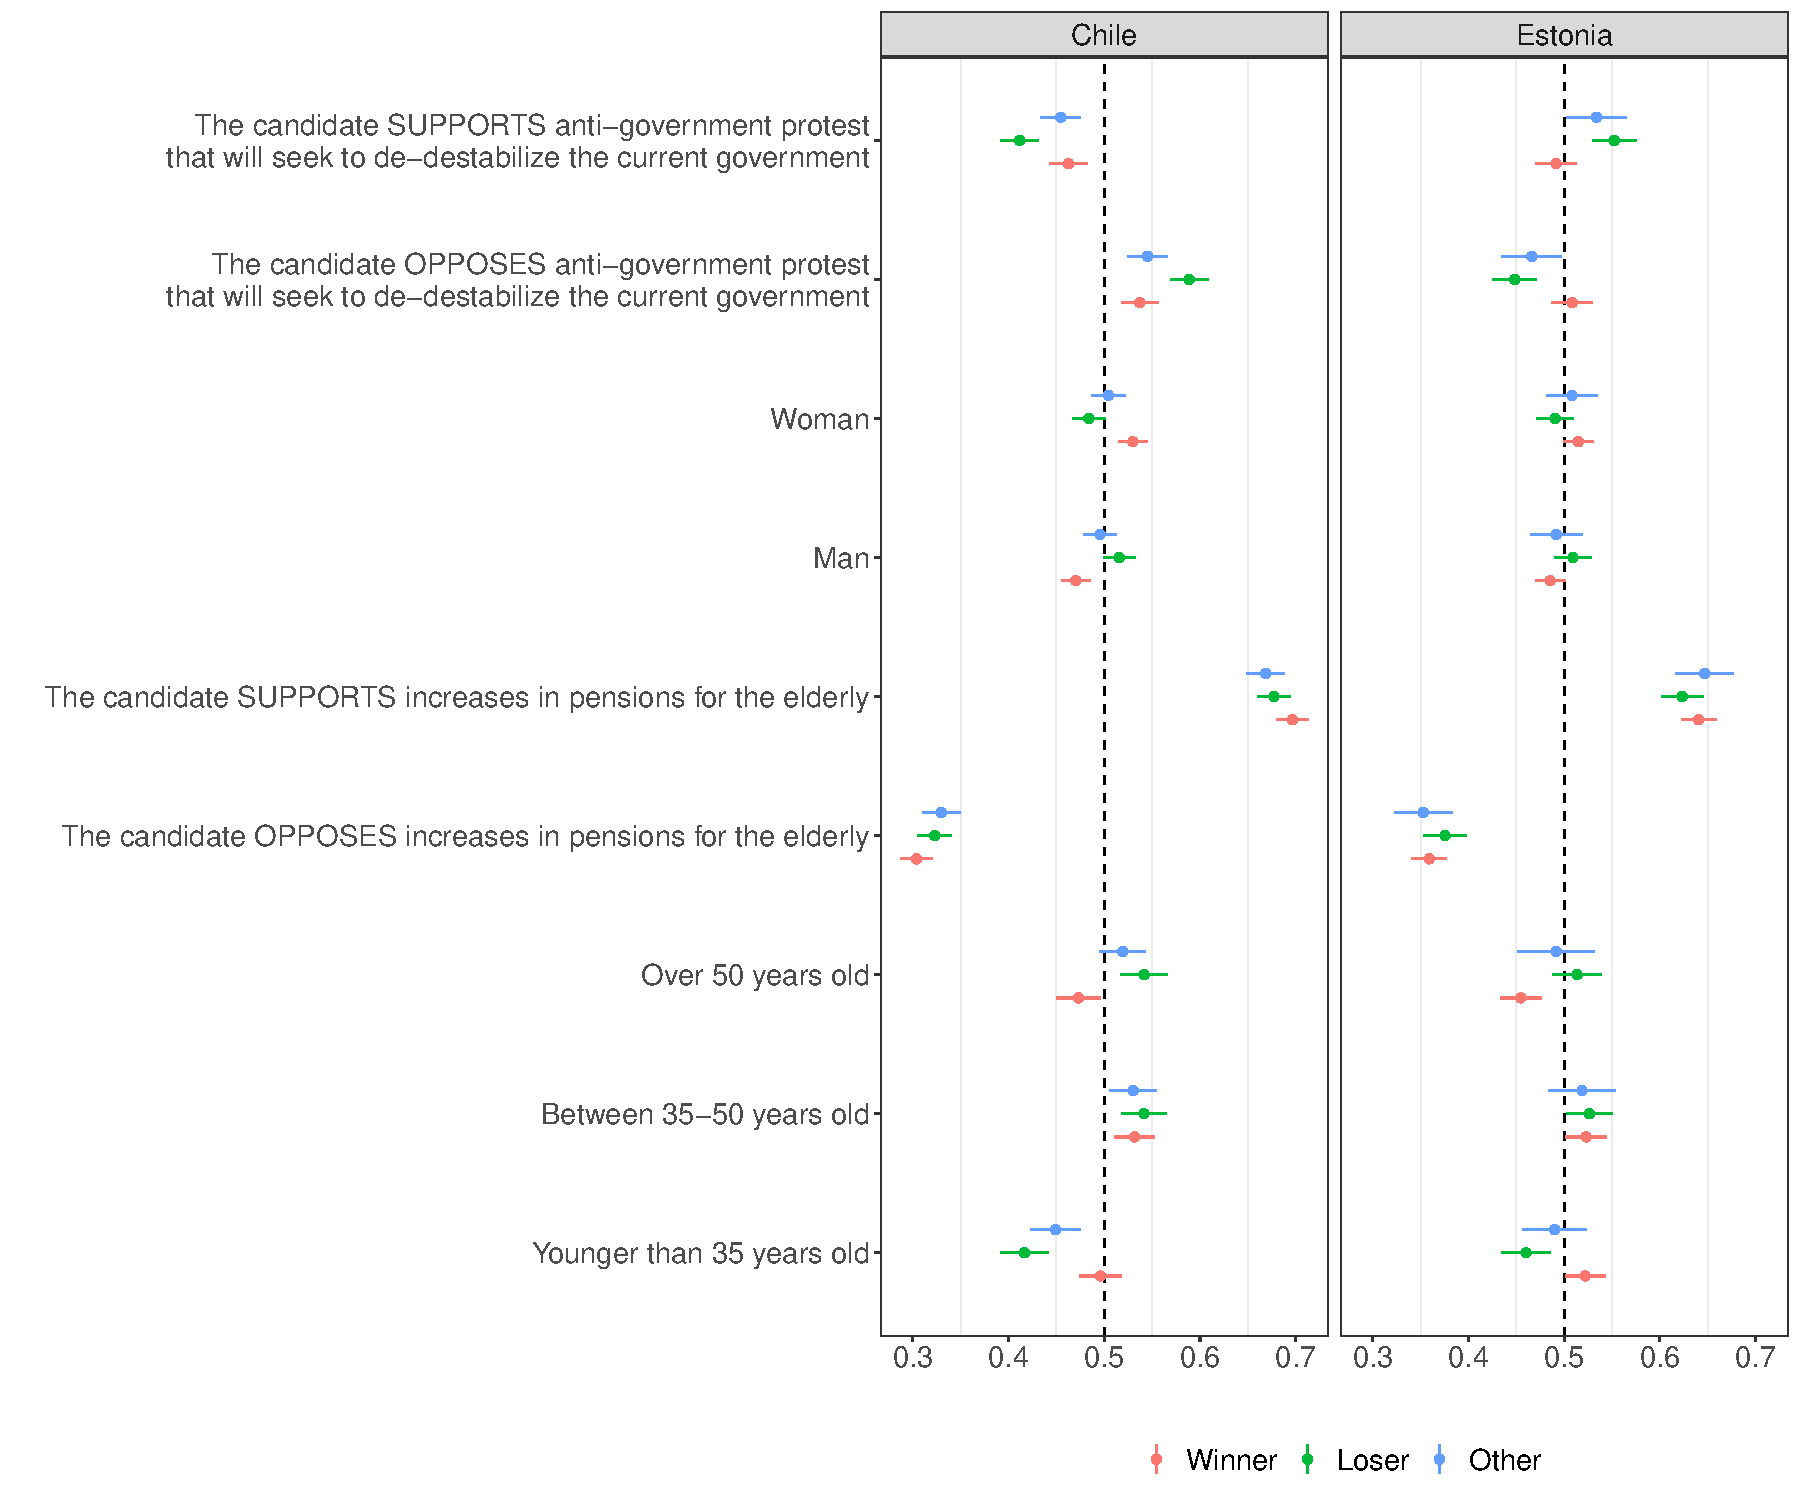
\includegraphics[scale=.295, center]{Conjoint_Winner_Loser.pdf}
        \end{center}
    \end{minipage}
\end{column}

\end{columns}

\end{frame}


\subsection{Subgroup Marginal Means (MM): Partisanship/Ideology}


\miniframeson
\begin{frame}[c]%{Losers' Consent and Democratic Stability}

\begin{columns}

\begin{column}[T]{0.35\textwidth}
    \begin{minipage}[c][.6\textheight][c]{\linewidth}
    \begin{itemize}
        \item {\only<2>{\leavevmode\color{Red}}Voters generally reject candidates favoring protests.}

        \item {\only<3>{\leavevmode\color{Red}}Extreme right voters (\emph{Rep. Party}) are especially likely to reject candidates associated with anti-systemic protest.}

        \item {\only<4>{\leavevmode\color{Red}}{\bf Estonia}: loser effects are largely driven by the extreme right}.


    \end{itemize} 
    \end{minipage}
\end{column}

\begin{column}[T]{0.7\textwidth}
    \begin{minipage}[c][.6\textheight][c]{1.1\linewidth}
        \begin{center}
          \vspace{0.6cm}\hspace{-0.8cm}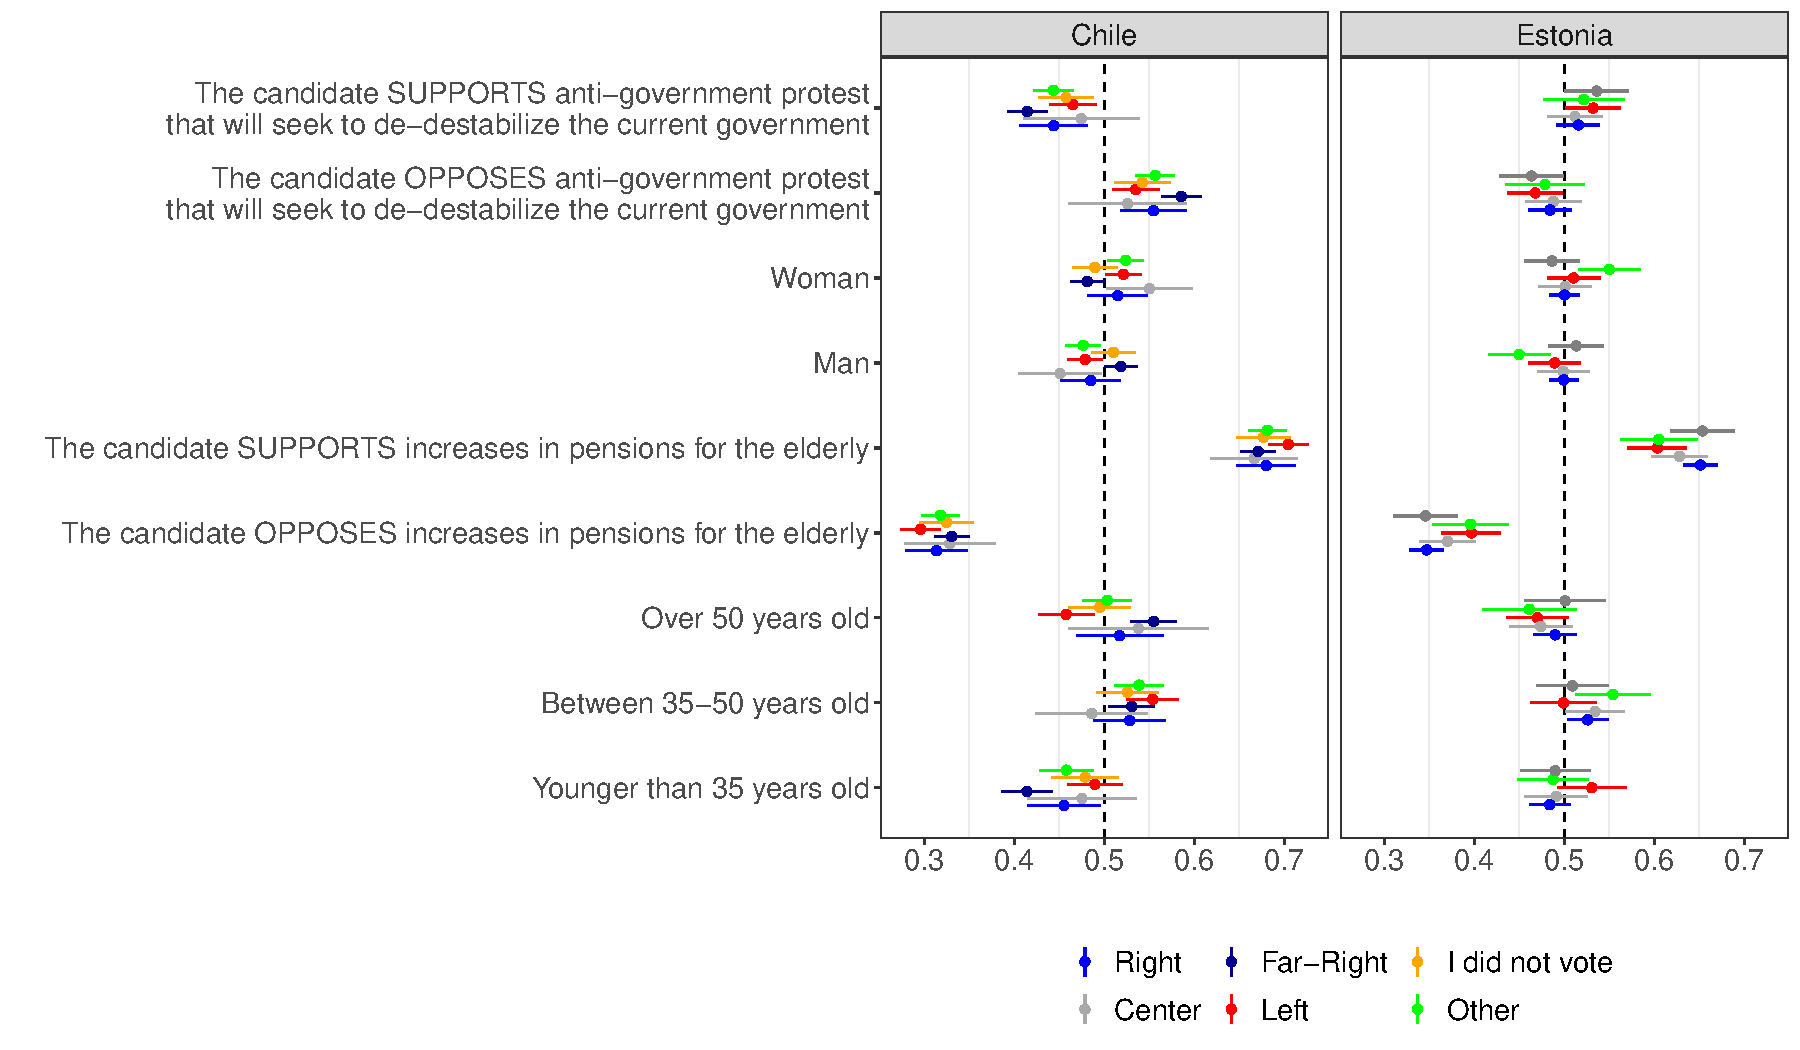
\includegraphics[scale=.2, center]{Conjoint_Vote_Choice.pdf}
        \end{center}
    \end{minipage}
\end{column}

\end{columns}

\end{frame}


\section{Discussion}


\subsection{Main Takeaways}



\miniframeson
\begin{frame}[c]{More Questions Than Answers}
  \begin{itemize}
    \item We hypothesized (and pre-registered) that:
      \begin{enumerate}
          \item[H1] \emph{Electoral losers} were \emph{more} willing to support anti-systemic protests. 
          \item[H2] This effect would be \emph{stronger} in Presidential systems \\ {\scriptsize(because of its zero-sum power sharing structure, {\bf losses are more catastrophic})}.
      \end{enumerate}
    
    \item While we did not find support in favor of our hypotheses, we still found some other interesting results.

    \begin{itemize}
      \item {\bf Chile}: {\color{blue}Extreme-right} supporters are {\color{blue}less} likely to support extreme anti-system protests.
      \item {\bf Estonia}: the {\color{blue}loser effects} are mainly {\color{blue}driven by extreme-right} supporters.
    \end{itemize}


    \item Did we make a mistake to think that, {\bf in Chile (!)}, right-wing losers were going to {\bf protests} (!)? {\bf Let me know what you think}.

  \end{itemize}
\end{frame}


\miniframesoff
\begin{frame}[c]{Thank you}
        \begin{center}
          \vspace{-0.7cm}\includegraphics[scale=.06, center]{/Users/hectorbahamonde/hbahamonde.github.io/resources/qr-code.pdf}
        \end{center}


        \begin{itemize}
            %\item Paper (draft) available at {\color{blue}www.HectorBahamonde.com}.
            \item[] {\large\color{red}\faCamera}\; to check updates on this project. 
        \end{itemize}
\end{frame}





\end{document}




                                                                                                                                                                               
